

\chapter{Prevalence estimation}

\section{The problem}

Consider a population of interest and a known condition, such as, for example,
a disease or a binary behavior. It is important to understand the proportion
of individuals in this population exposed at time $t$, called {\em
prevalence}. Suppose a diagnostic test is done to measure the presence or the
absence of this condition in the individuals. Mathematically, let $\theta \in
(0,1)$ be the prevalence (parameter of interest) of the condition and $Y_i$ be an indicator function of the presence of the condition in the i$^{th}$ individual.
Assuming for simplicity that all tests are performed at time $t$, and the
sample is $\{y_1, ..., y_n\}$, the maximum likelihood estimator is the
apparent prevalence: 
\begin{equation}
    \label{eq:naive-estimator}
    \hat{\theta} = \frac{1}{n}\sum_{i=1}^n y_i.
\end{equation}
However, this estimator has two problems in this context: it assumes a perfect
diagnostic test, which is often incorrect, and the samples in RDS are not
independent by definition (network structure). 

The first problem in \eqref{eq:naive-estimator} was tackled several times in
the literature, such as \cite{mcinturff2004modelling}. The diagnose accuracy
can be measured in many ways and the most considered is the joint analysis of
the {\em sensitivity} ($\gamma_s$) and the {\em specificity}
($\gamma_e$). 

\begin{definition}[Specificity]
    It is the probability of a negative test conditioned on the absence of the
    disease (true negative).
\end{definition}

\begin{definition}[Sensitivity]
    It is the probability of a positive test conditioned on the presence of
    the disease (true positive). 
\end{definition}

Let $p$ be the probability of a positive test. Then, by Law of Total
Probability: 
\begin{equation}
    p = \theta\gamma_s + (1-\theta)(1-\gamma_e).    
\end{equation}

Assuming the tests are conditionally independent given the presence or the
absence of the disease in each individual, the number of positive tests $X$
has binomial distribution with success probability $p$. In chapter
XXX we present preliminary model that
accounts this.  Regression approaches can be also carried with a link function
in $\theta$. One important additional problem is to consider the
correlation between $\gamma_s$ and $\gamma_e$. 


The second problem was a study object in \cite{heckathorn1997,heckathorn2002} where the estimator was proposed
based largely on Markov chain theory and social network theory.
\cite{volz2008probability} improved it with the RDS II estimator considering
the network degree
\begin{equation}
    \hat{\theta}^{RDS II} = \frac{\sum_{i=1}^n y_i \delta_i^{-1}}{\sum_{i=1}^n \delta_i^{-1}},
\end{equation}
such that $\delta_i$ is the i$^{th}$ individual's degree. However, this is an
area of research in progress. 



Let $I$ be a index set and $Y_i$ be the indicator function of the $i^{th}$ individual's exposure to the disease, and $T_i$
indicating whether the test of the $i^{th}$ individual is positive at time
$t$. Suppose that $\{Y_i\}_{i \in I}$ and $\{T_i\}_{i \in I}$ are two independent and identically distributed
random variables with $\Pr(X = 1) = \theta$ and $\Pr(T = 1) = p$. We say that
$\theta$ is the prevalence and $p$ is the apparent prevalence in the
population. 

If the test is perfect, then for every $i$, $T_i = Y_i$, and
$\theta = p$ (with probability one when they are random variables).
Unfortunately, this is not true in the real world, what makes important to
regard the evaluation of the diagnostic, and the following definitions are used:

\begin{definition}[Specificity]
  Probability of a negative test correctly identified. In mathematical terms,
  conditioned on $Y = 0$, the {\em specificity} $\gamma_e$ is the probability of $T = 0$: 
  \begin{equation}
    \gamma_e = \Pr(T = 0|Y = 0). 
  \end{equation} 
\end{definition}

\begin{definition}[Sensitivity]
  Probability of a positive test correctly identified. In mathematical terms,
  conditioned on $Y = 1$, the {\em sensitivity} $\gamma_s$ is the probability of $T = 1$: 
  \begin{equation}
    \gamma_s = \Pr(T = 1|Y = 1). 
  \end{equation} 
\end{definition}

\begin{theorem}[Relation between prevalence and apparent prevalence] These quantities are related by the following equation:
  \begin{equation}
    p = \gamma_s\theta + (1-\gamma_e)(1-\theta).
  \end{equation}
  
\end{theorem}

\begin{proof}
  This is a direct application of the definition of conditional probability
  and the countable additivity axiom of Probability:
  \begin{equation*}
    \begin{split}
      p &= \Pr(T = 1) = \Pr(T = 1, Y = 1) + \Pr(T = 1, Y = 0) \\
      &= \Pr(T=1|Y=1)\Pr(Y=1) + \Pr(T=1|Y=0)\Pr(Y=0) \\
      &= \Pr(T=1|Y=1)\Pr(Y=1) + (1 - \Pr(T=0|Y=0))(1-\Pr(Y=1)) \\
      &= \gamma_s\theta + (1 - \gamma_e)(1-\theta).
    \end{split}
  \end{equation*} 
\end{proof}

The intuition behind this equation is pretty simple: the proportion
of positive test counts the correct identified exposed individuals and the
incorrect identified not exposed. Observe that if $\gamma_s = \gamma_e = 1$, we have the trivial case $p =
\theta$. Moreover, if $\gamma_s = \gamma_e = 0.5$, we have that
$p = 0.5$ and there is no information about $\theta$. 

\begin{remark}
  Actually, we are interested in the prevalence at time $t$. When it is 
  impossible to test every individual at the same time, we assume that all
  individuals remain exposed to the disease at time of the last tested individual. 
\end{remark}

\improve{\begin{definition}[Link function]
  A class of functions which maps a non-linear relationship to a linear one.
  Here we consider functions with domain $[0,1]$. Examples include the logit
  and probit functions.
\end{definition}}

\section{Model approach for prevalence estimation}

Firstly, we make some assumptions to simplify the modeling:

\begin{assumption}  
  For a Bayesian modeling, we assume each model's parameter has a probability distribution that incorporates the researcher's uncertainty about it. 
\end{assumption}

\begin{assumption}
  For each individual, we observe $k$ regressors that are possible
  risk factors represented by the vector $\x_i \in \R^{k}$ of the $i^{th}$
  individual. We assume that the probability $\theta_i$ of the $i^{th}$ individual having been exposed
  to the disease dependes on the prevalence $\theta$ and $\x_i$. The
  probability of positive test in the $i^{th}$ individual is denoted by $p_i$. Therefore, the sequences $\{Y_i\}_{i \in I}$ and $\{T_i\}_{i \in I}$ are not
  identically distributed anymore.
\end{assumption}

\begin{assumption}
  Sensitivity and specificity have the same distribution for all
  individuals and it only depends on the test used to diagnose. 
\end{assumption}

From above, we develop three different models.

\subsection{Perfect tests}

The first model supposes the samples are independent and the test is perfect,
which means that $\theta_i = p_i$ for all $i$. Therefore it only considers the risk factors $\x_i$. 

\begin{equation}
  \begin{aligned}
    T_i &\sim \bern(\theta_i), \\
    g(\theta_i) &= g(\theta) + \x_i^T\beta, 
  \end{aligned}  
\end{equation}
where $v^T$ denotes the transpose of $v$, and $g(\cdot)$ is a link function.
The parameter $\beta \in \R^{k}$ is the risk effects. For Bayesian inference, priors on
$\beta$ and $\theta$ must be included. We use $\beta ~ \sim \N(\mu, \Sigma)$
and $\theta \sim \betadist(a^{p}, b^p)$, where $\mu
\in \R^{k}$, $\Sigma \in \R^{k\times k}$ symmetric positive-definite matrix,
$a^p \in \R_{++}$, and $b^p \in \R_{++}$
are fixed hyperparameters. 

\begin{remark}
  If the risk factors are zero, i.e $\x_i = 0$, the probability of the
  $i^{th}$ having been exposed is the prevalence $\theta$, which means that in
  a population with no risk effects, the probability of a person has the
  disease is exactly the proportion in this population. 
\end{remark}

\subsubsection{Identifiability}

\subsubsection{Experiments}

\url{https://github.com/lucasmoschen/rds-bayesian-analysis/blob/main/exercises/primary_model/model_experiments.ipynb}

\subsection{Imperfect tests}

This model includes the sensitivity and specificity of the diagnostic test. 

\begin{equation}
  \begin{aligned}
    T_i &\sim \bern(p_i) \\
    p_i &= \gamma_s\theta_i + (1-\gamma_e)(1 - \theta_i),  \\
    g(\theta_i) &= g(\theta) + \x_i^T\beta,  \\
    \beta &\sim \N(\mu, \Sigma), \\ 
    \theta &\sim \betadist(a^p, b^p) \\
    \gamma_s &\sim \betadist(a^s, b^s), \\
    \gamma_e &\sim \betadist(a^e, b^e), \\    
  \end{aligned}  
\end{equation}
where $a^p, a^s, a^e, b^p, b^s, b^e \in \R_{++}$ are fixed hyperparameters.
This model does not include prior knowledge about the correlation between
specificity and sensitivity. 

\subsubsection{Experiments}

Consider the following model \cite{gelman2020bayesian}:
\begin{gather*}
  y \sim \operatorname{Binomial}(n, p), \\
  p = \theta\gamma_s + (1- \theta)(1-\gamma_e), 
\end{gather*}
such that $y$ is the number of positive tests in a population of size $n$. In
a Bayesian paradigm, a prior $\pi(\theta, \gamma_e, \gamma_s)$ must be
specified. For instance, $\pi(\theta, \gamma_e, \gamma_s) =
\pi(\theta)\pi(\gamma_e, \gamma_s)$ and $\theta \sim
\operatorname{Beta}(\alpha_{\theta}, \beta_{\theta})$, in which
$\alpha_{\theta}$ and $\beta_{\theta}$ are positive hyperparameters. Since the
three parameters $\theta, \gamma_e$, and $\gamma_s$ are not jointly
identifiable only from $y$, prior information on $\gamma_e$ and $\gamma_s$
need be added. For this, 
\begin{gather*}
  y_{negative} \sim \operatorname{Binomial}(n_{\gamma_e}, \gamma_e), \\
  y_{positive} \sim \operatorname{Binomial}(n_{\gamma_s}, \gamma_s),
\end{gather*}
such that $y_{negative}$ are negative tests on known negative subjects
(by a gold standard for example) and $y_{positive}$ are positive tests on
known positive. When considering separated experiments for specificity and
sensitivity, there is
no information about their correlation, which is the case for our model. Then we define the the prior distributions
\begin{gather*}
  \gamma_e \sim \operatorname{Beta}(a_e, b_e), \\
  \gamma_s \sim \operatorname{Beta}(a_s, b_s), \\
  \theta \sim \operatorname{Beta}(a_{\theta}, b_{\theta}).
\end{gather*} 
Using data from \cite{bennett2020estimating} about COVID-19 seroprevalence in
Santa Clara:  
\begin{align*}
  y/n &= 50/3330,\\
y_{negative}/n_{\gamma_e} &= 399/401, \\
y_{positive}/n_{\gamma_s} &= 103/122, 
\end{align*}
we fit the model and obtain the results showed in Figure
\ref{fig:results-posterior-model1}. All the codes were done in {\em Stan} and
{\em PyStan}.

\begin{figure}[!ht]
  \centering
  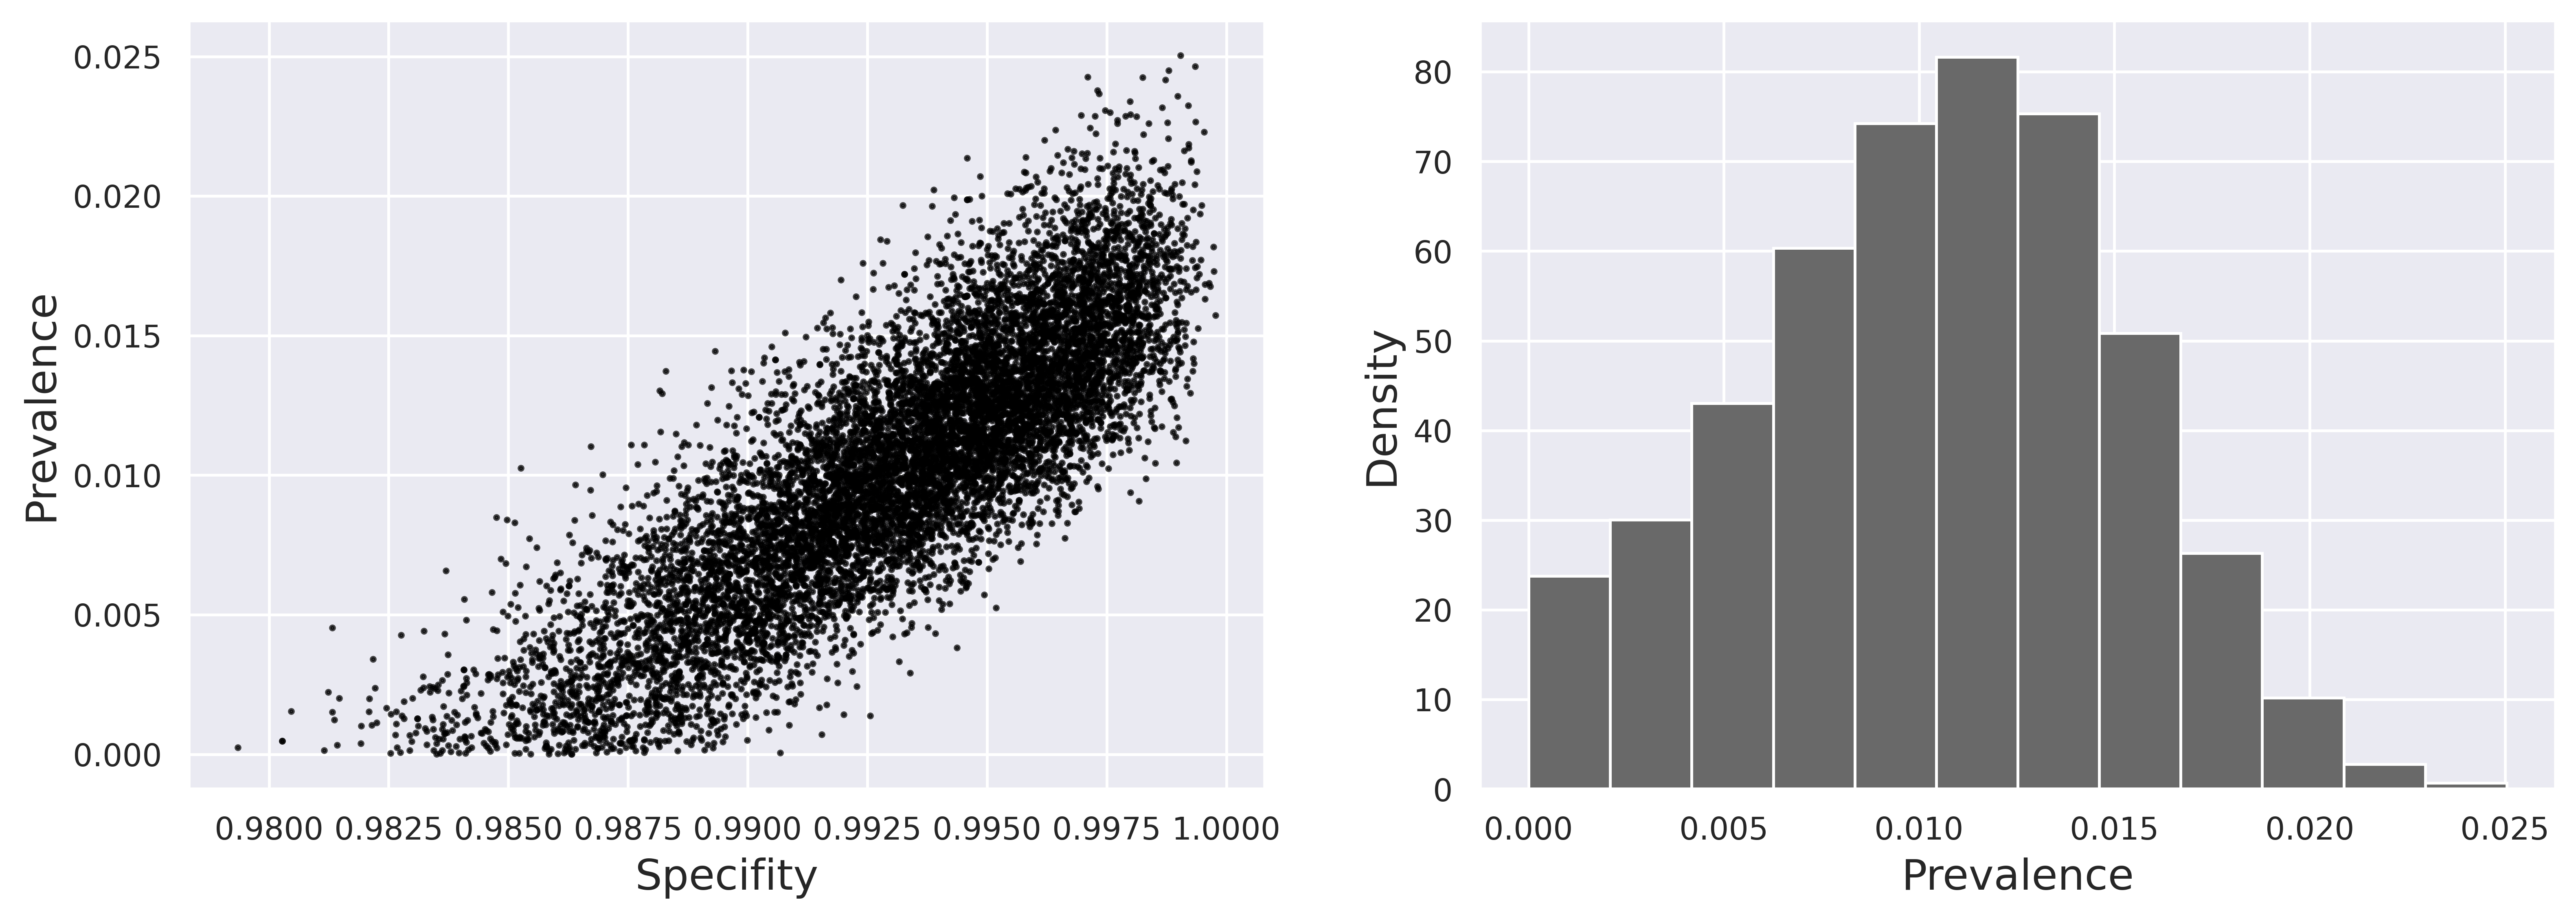
\includegraphics[width=\textwidth]{../../images/model1_gelman_figure_english.png}
  \caption{Scatter plot of posterior simulations of prevalence against
  specificity and histogram of posterior simulations of the prevalence.}
  \label{fig:results-posterior-model1}
\end{figure}

Other approach considers more than one study about specificity and
sensitivity. A {\em hierarchical partial pooling} model for these studies
can be done in the following way: 
\begin{gather*}
    \operatorname{logit}(\gamma_s^j) \sim \operatorname{Normal}(\mu_{\gamma_s}, \sigma_{\gamma_s}), \\
    \operatorname{logit}(\gamma_e^j) \sim \operatorname{Normal}(\mu_{\gamma_e}, \sigma_{\gamma_e}), 
\end{gather*}
for $1 \le j \le K$ studies, such that the first study is the considered one.
Partial pooling because the parameters can be sampled from the same
distribution. Hierarchical because the parameters of this distribution have
its one prior distributions. For instance, 
\begin{align*}
    \mu_{\gamma_s} &\sim N(0, 10), \\ 
    \mu_{\gamma_e} &\sim N(0, 10), \\
    \sigma_{\gamma_s} &\sim N^+(0,1), \text{ and } \\
    \sigma_{\gamma_e} &\sim N^+(0,1),
\end{align*}
where $N^+(a,b)$ is the truncated normal distribution in $[0,+\infty)$. All
the codes available at Github
repository\footnote{\url{https://github.com/lucasmoschen/rds-bayesian-analysis}}.

Finally, we studied a joint distribution for specificity and sensitivity, a
possible bivariate beta distribution built in \cite{olkin2015constructions}.
This distribution is derived from a Dirichlet distribution of order four. Let $U = (U[1],...,U[4]) \sim \operatorname{Dirichlet}(\boldsymbol{\alpha})$, where
$\boldsymbol{\alpha} \in \mathbb{R}^4_+$. Therefore, defining $X = U[1] +
U[2]$ and $Y = U[1] + U[3]$, we will have that $(X,Y)$ has a well-defined
probability distribution in
$[0,1] \times [0,1]$ such that $X$ and $Y$ have marginally beta distributions,
and they have correlation in all space. Depending on the definition of
$\boldsymbol{\alpha}$, the correlation between the variables range from -1 and
1. Figure \ref{fig:beta-bivariate} shows some examples of this construction. 

\begin{figure}[!ht]
    \centering
    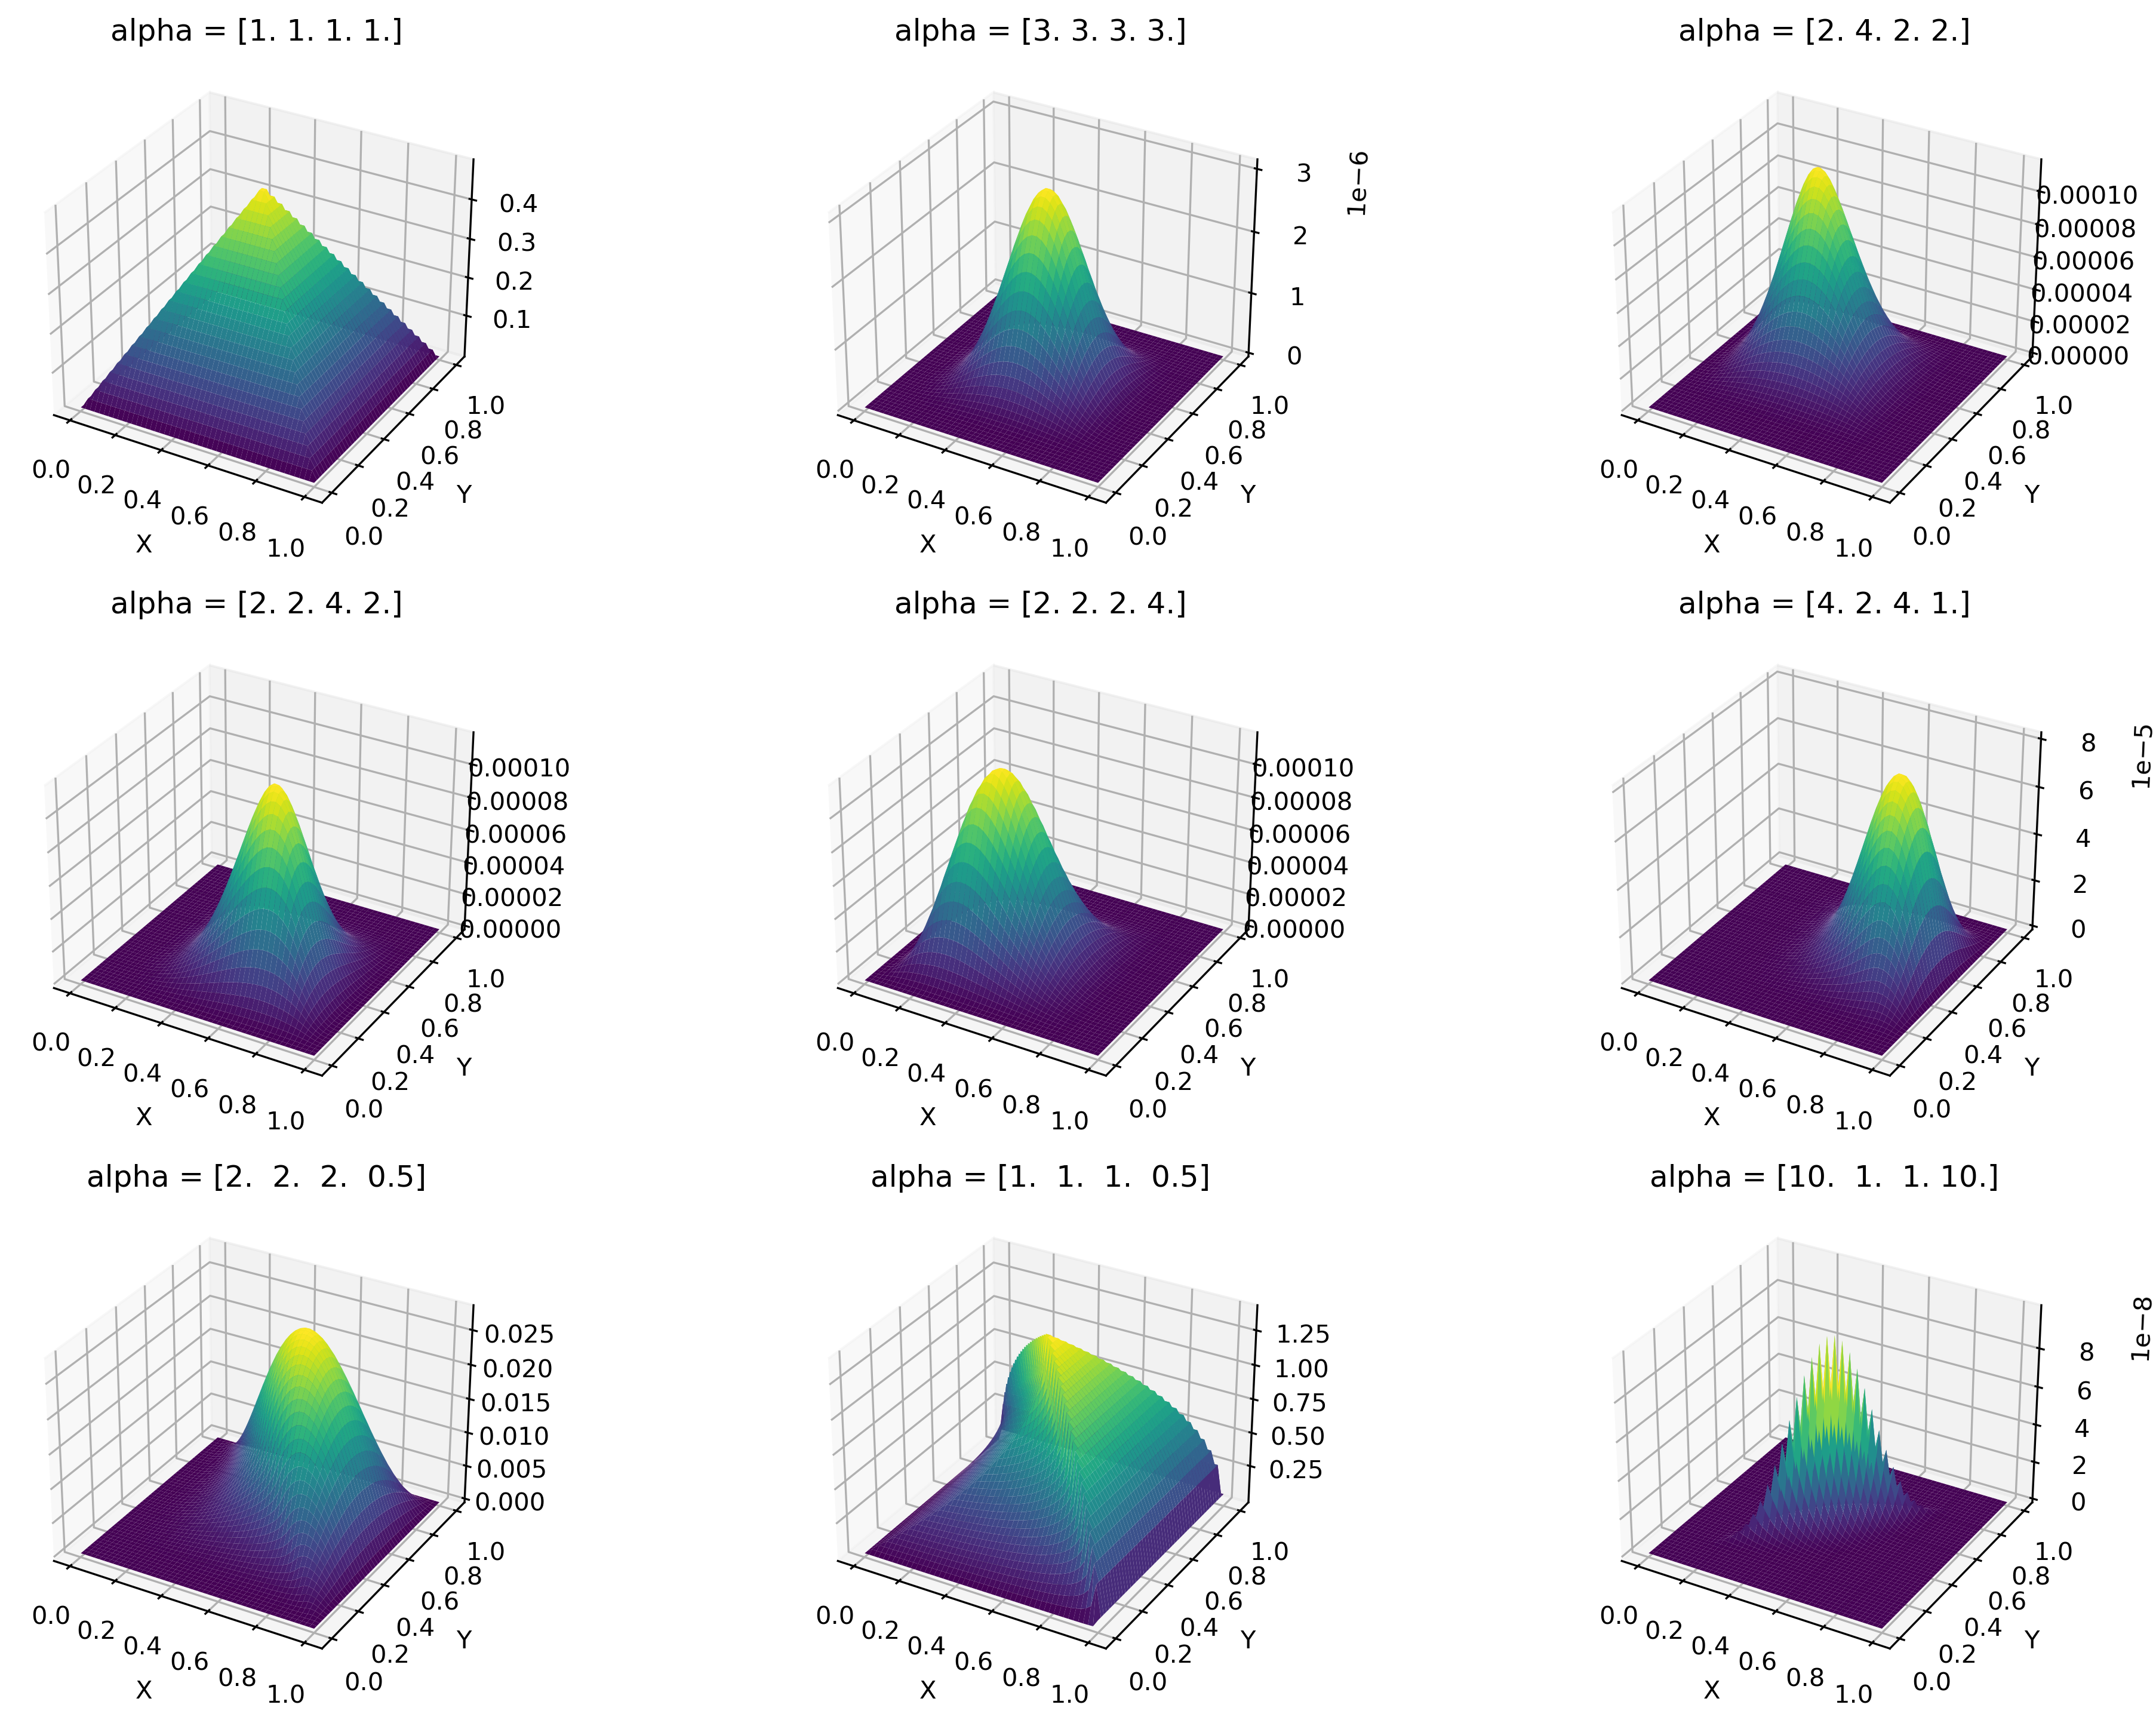
\includegraphics[width=\textwidth]{beta-distributions.png}
    \caption{Different choices of $\alpha$ and the joint distribution of the variables $X$ and $Y$.}
    \label{fig:beta-bivariate}
\end{figure}

\subsection{Imperfect tests and respondent-driven sampling}

For now, we consider the network dependence induced by the RDS with no
associated model. Therefore, we treat it as a random effect for
each individual. Conditionally autoregressive (CAR) models in the
Gaussian case are used. Let $[\tilde{Q}]_{ij} = \tilde{q}_{ij}$ be a fixed matrix which measures the distance between $i$
and $j$, and $\tilde{q}_{i+} = \sum_{j} \tilde{q}_{ij}$. In general, we use
$$
\tilde{q}_{ij} = \begin{cases}
  1, &\text{if } i \text{ recruited } j \text{ or the contrary} \\
  0, &\text{otherwise.} 
\end{cases}
$$
Next we define the scaled adjacency matrix $Q = D^{-1}\tilde{Q}$, such that $D$
is a diagonal matrix with $D_{ii} = \tilde{q}_{i+}$. Finally let $|\rho| < 1$ be a
parameter to controls the dependence between neighbors. Hence, we specify the
model as follows:

\begin{equation}
  \begin{aligned}
    T_i &\sim \bern(p_i) \\
    p_i &= \gamma_s\theta_i + (1-\gamma_e)(1 - \theta_i),  \\
    g(\theta_i) &= g(\theta) + \x_i^T\beta + \omega_i,  \\
    \omega_i|\{\omega_j\}_{j\neq i}, \tau &\sim \N\left(\rho\sum_j q_{ij}\omega_j, \tau^{-1}/\tilde{q}_{i+}\right) \\
    \beta &\sim \N(\mu, \Sigma), \\ 
    \theta &\sim \betadist(a^p, b^p) \\
    \gamma_s &\sim \betadist(a^s, b^s), \\
    \gamma_e &\sim \betadist(a^e, b^e), \\  
    \tau &\sim \operatorname{Gamma}(a^{\tau}, b^{\tau}).
  \end{aligned}  
\end{equation}
By Brook's Lemma \cite[]{brook1964distinction}, the joint distribution of
$\omega$ can be specified as 
$$
\omega \sim \N\left(0, \left[\tau (D - \rho \tilde{Q})\right]^{-1}\right).
$$

\subsubsection{Exponential Random Graph Model (ERGM)}

RDS has the constraint of being without replacement. For that reason, we do
not observe all links among the samples \cite[]{crawford2016}. Considering the
model developed by Crawford, we can model the
matrix $Q$ as {\em Exponential Random Graph Model} (ERGM). Define the
following 

\begin{enumerate}
  \item $\boldsymbol{s} = \tril(QC)^T \boldsymbol{1} + C^Tu$, such that $Q$ is the
  adjacency matrix of the recruited subjects, $C$ is the {\em Coupon Matrix},
  $u$ the vector of the number of edge ends belonging to each vertex
  (in the order of recruitment) that are not connected to any other sampled
  vertex, and $\tril(M)$ the lower triangle of $M$. 

  \item $T(Q) = -\lambda \boldsymbol{s}$, such that $\lambda$ is the rate of
  the recruitment time. 

  \item $V(Q) = \sum_{k \text{ is not seed}} \log(\lambda \boldsymbol{s}_k)$
  
  \item $w = (0, t_2 - t_1, ..., t_n - t_{n-1})$ is the vector of the waiting times between
  recruitments.  
\end{enumerate}

Therefore $\Pr(Q|w) \propto \exp[T(Q)^Tw + V(Q)]$. With that, the model
becomes 

\begin{equation}
  \begin{aligned}
    T_i &\sim \bern(p_i) \\
    p_i &= \gamma_s\theta_i + (1-\gamma_e)(1 - \theta_i),  \\
    g(\theta_i) &= g(\theta) + \x_i^T\beta + \omega_i,  \\
    \omega_i|\{\omega_j\}_{j\neq i}, \tau &\sim \N\left(\rho\sum_j q_{ij}\omega_j/q_{i+}, \tau^2/q_{i+}\right) \\
    Q|w &\propto \exp[T(Q)^Tw + V(Q)] \\
    \lambda &\sim \Gamma(a^{\lambda}, b^{\lambda}), \\ 
    \beta &\sim \N(\mu, \Sigma), \\ 
    \theta &\sim \betadist(a^p, b^p) \\
    \gamma_s &\sim \betadist(a^s, b^s), \\
    \gamma_e &\sim \betadist(a^e, b^e), \\  
    \tau &\sim \N^+(0,\sigma^2_{\tau}).
  \end{aligned}  
\end{equation}
The problem with this model is that we are assigning a posterior distribution
for $Q$.